\section{Messprotokolle}

\begin{figure}[h!]
 \centering
 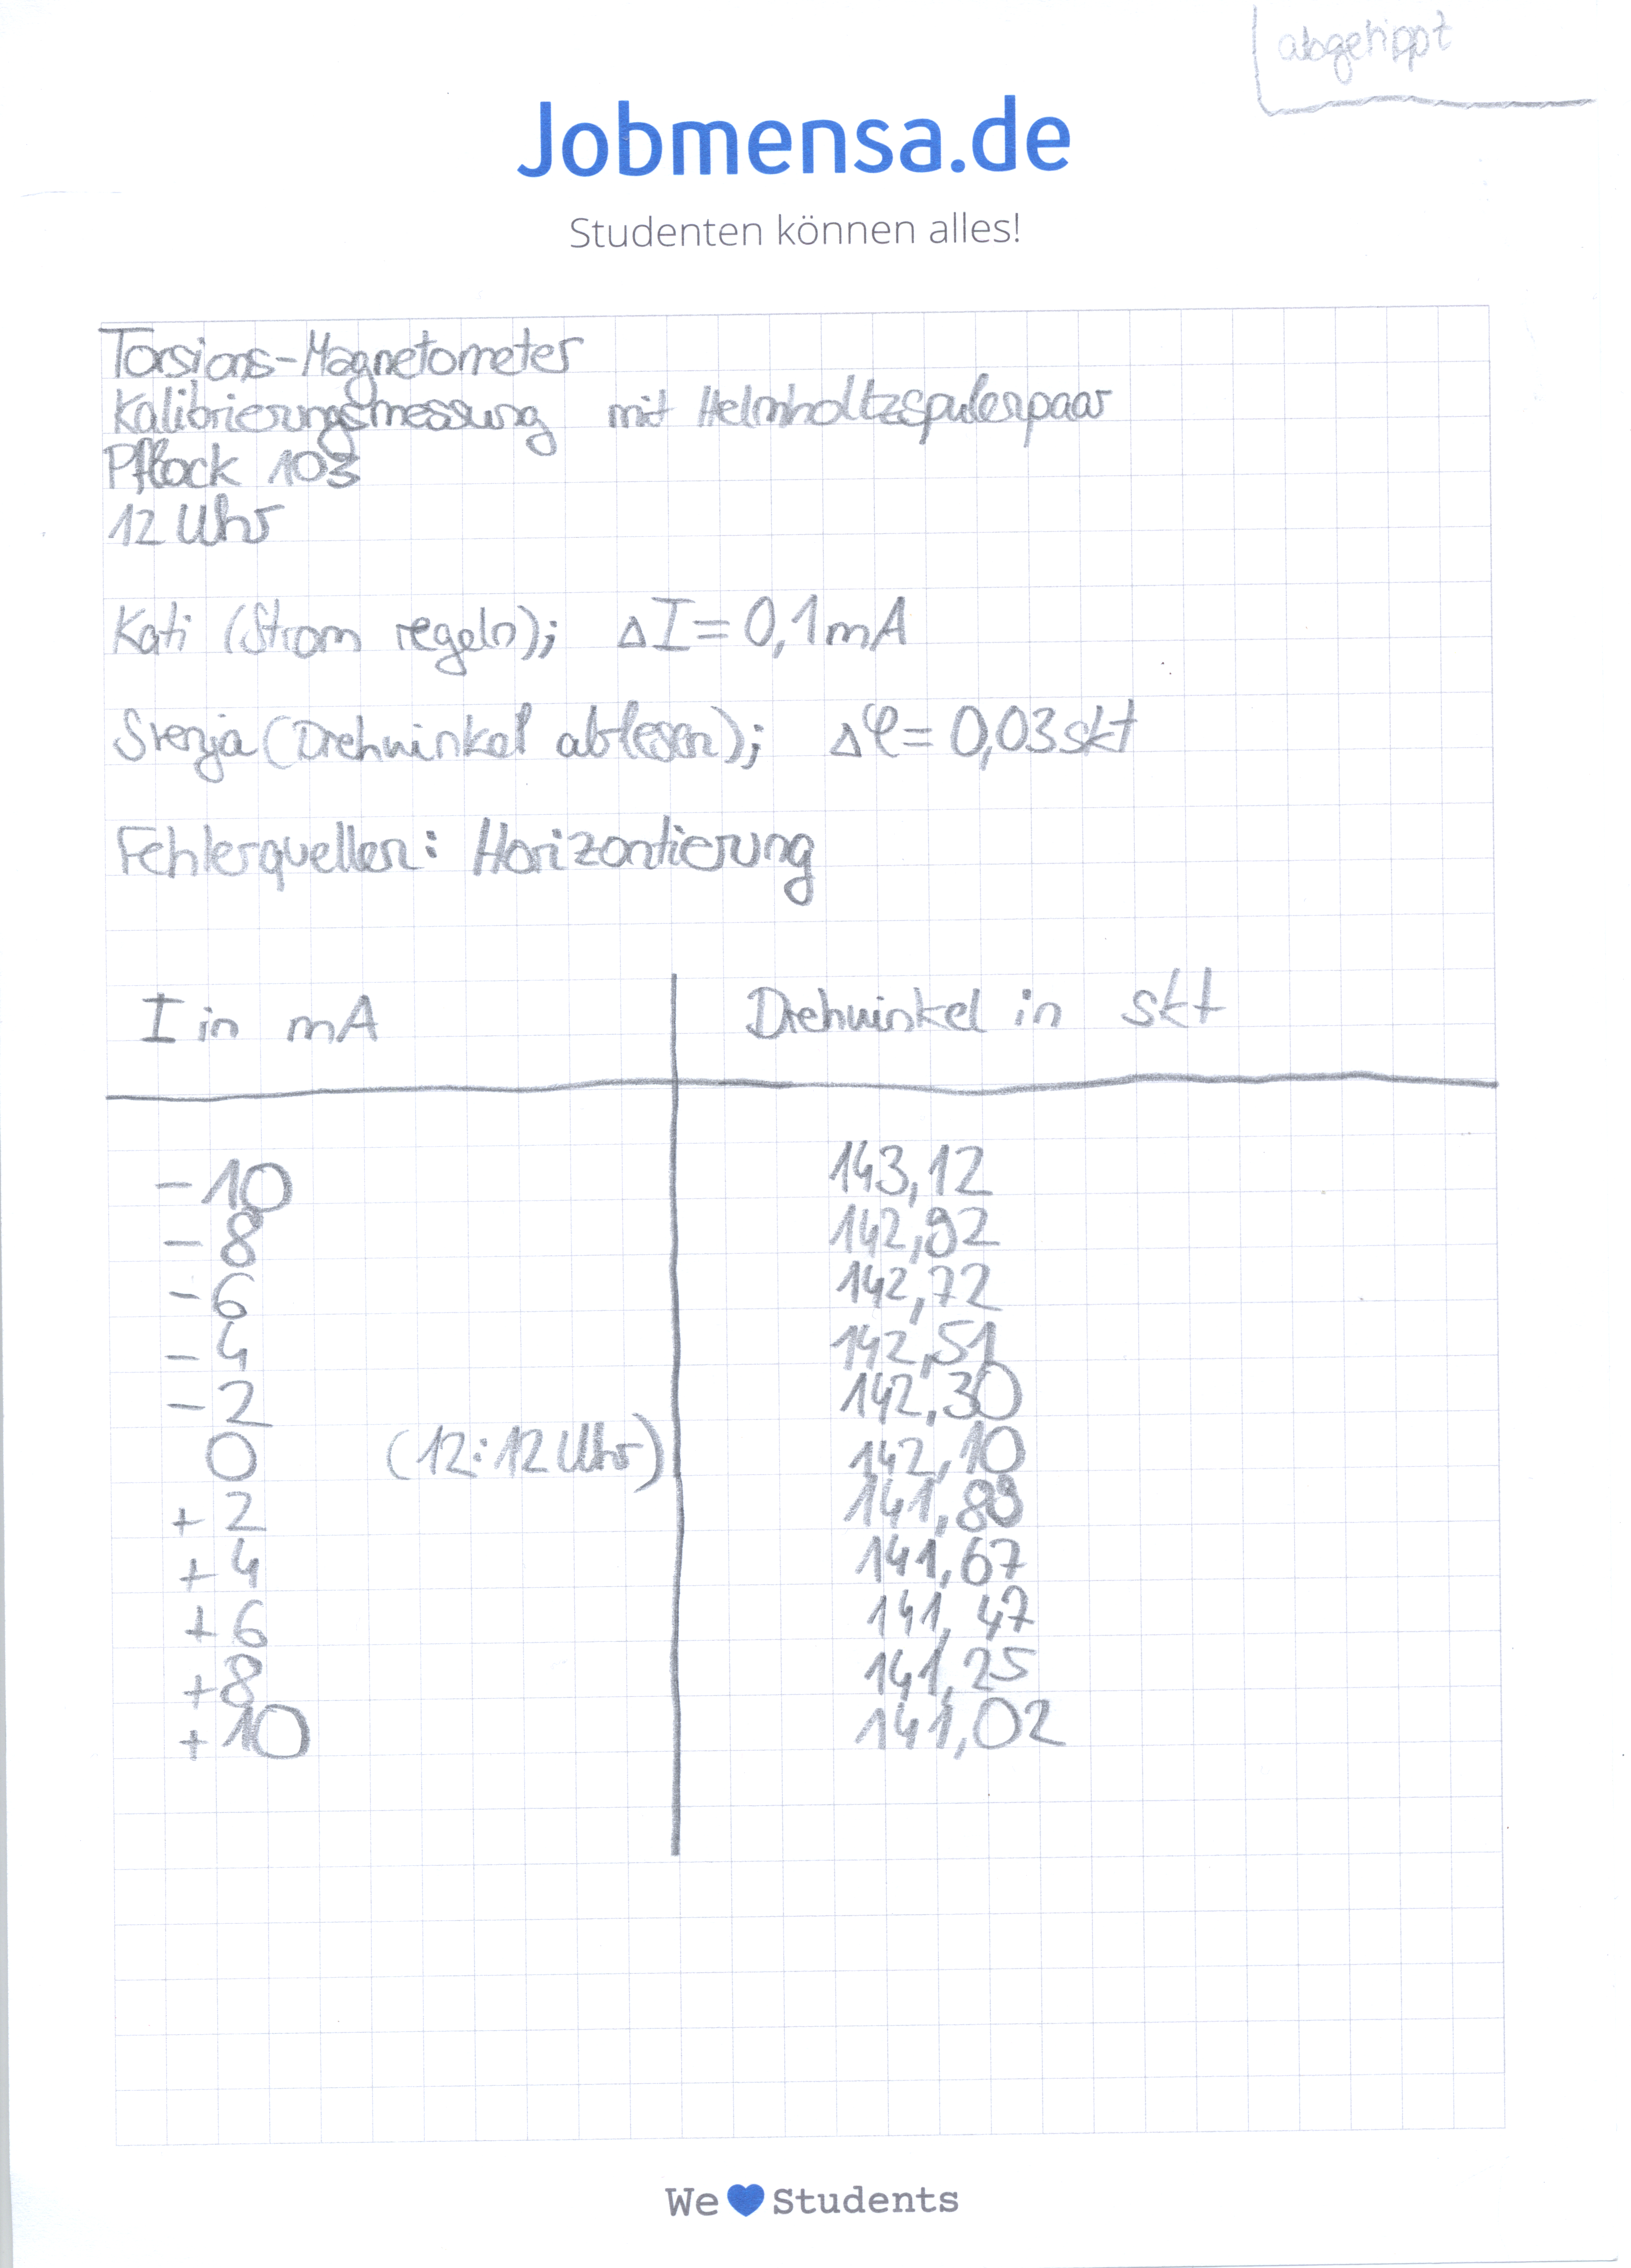
\includegraphics[width=0.8\textwidth]{fig/Messprotokolle/Kalibrierung.png}
 \caption{Messprotokoll zur Kalibrierungsmessung}
 \label{fig:MPKalibrierung}
\end{figure}

\begin{figure}[h!]
 \centering
 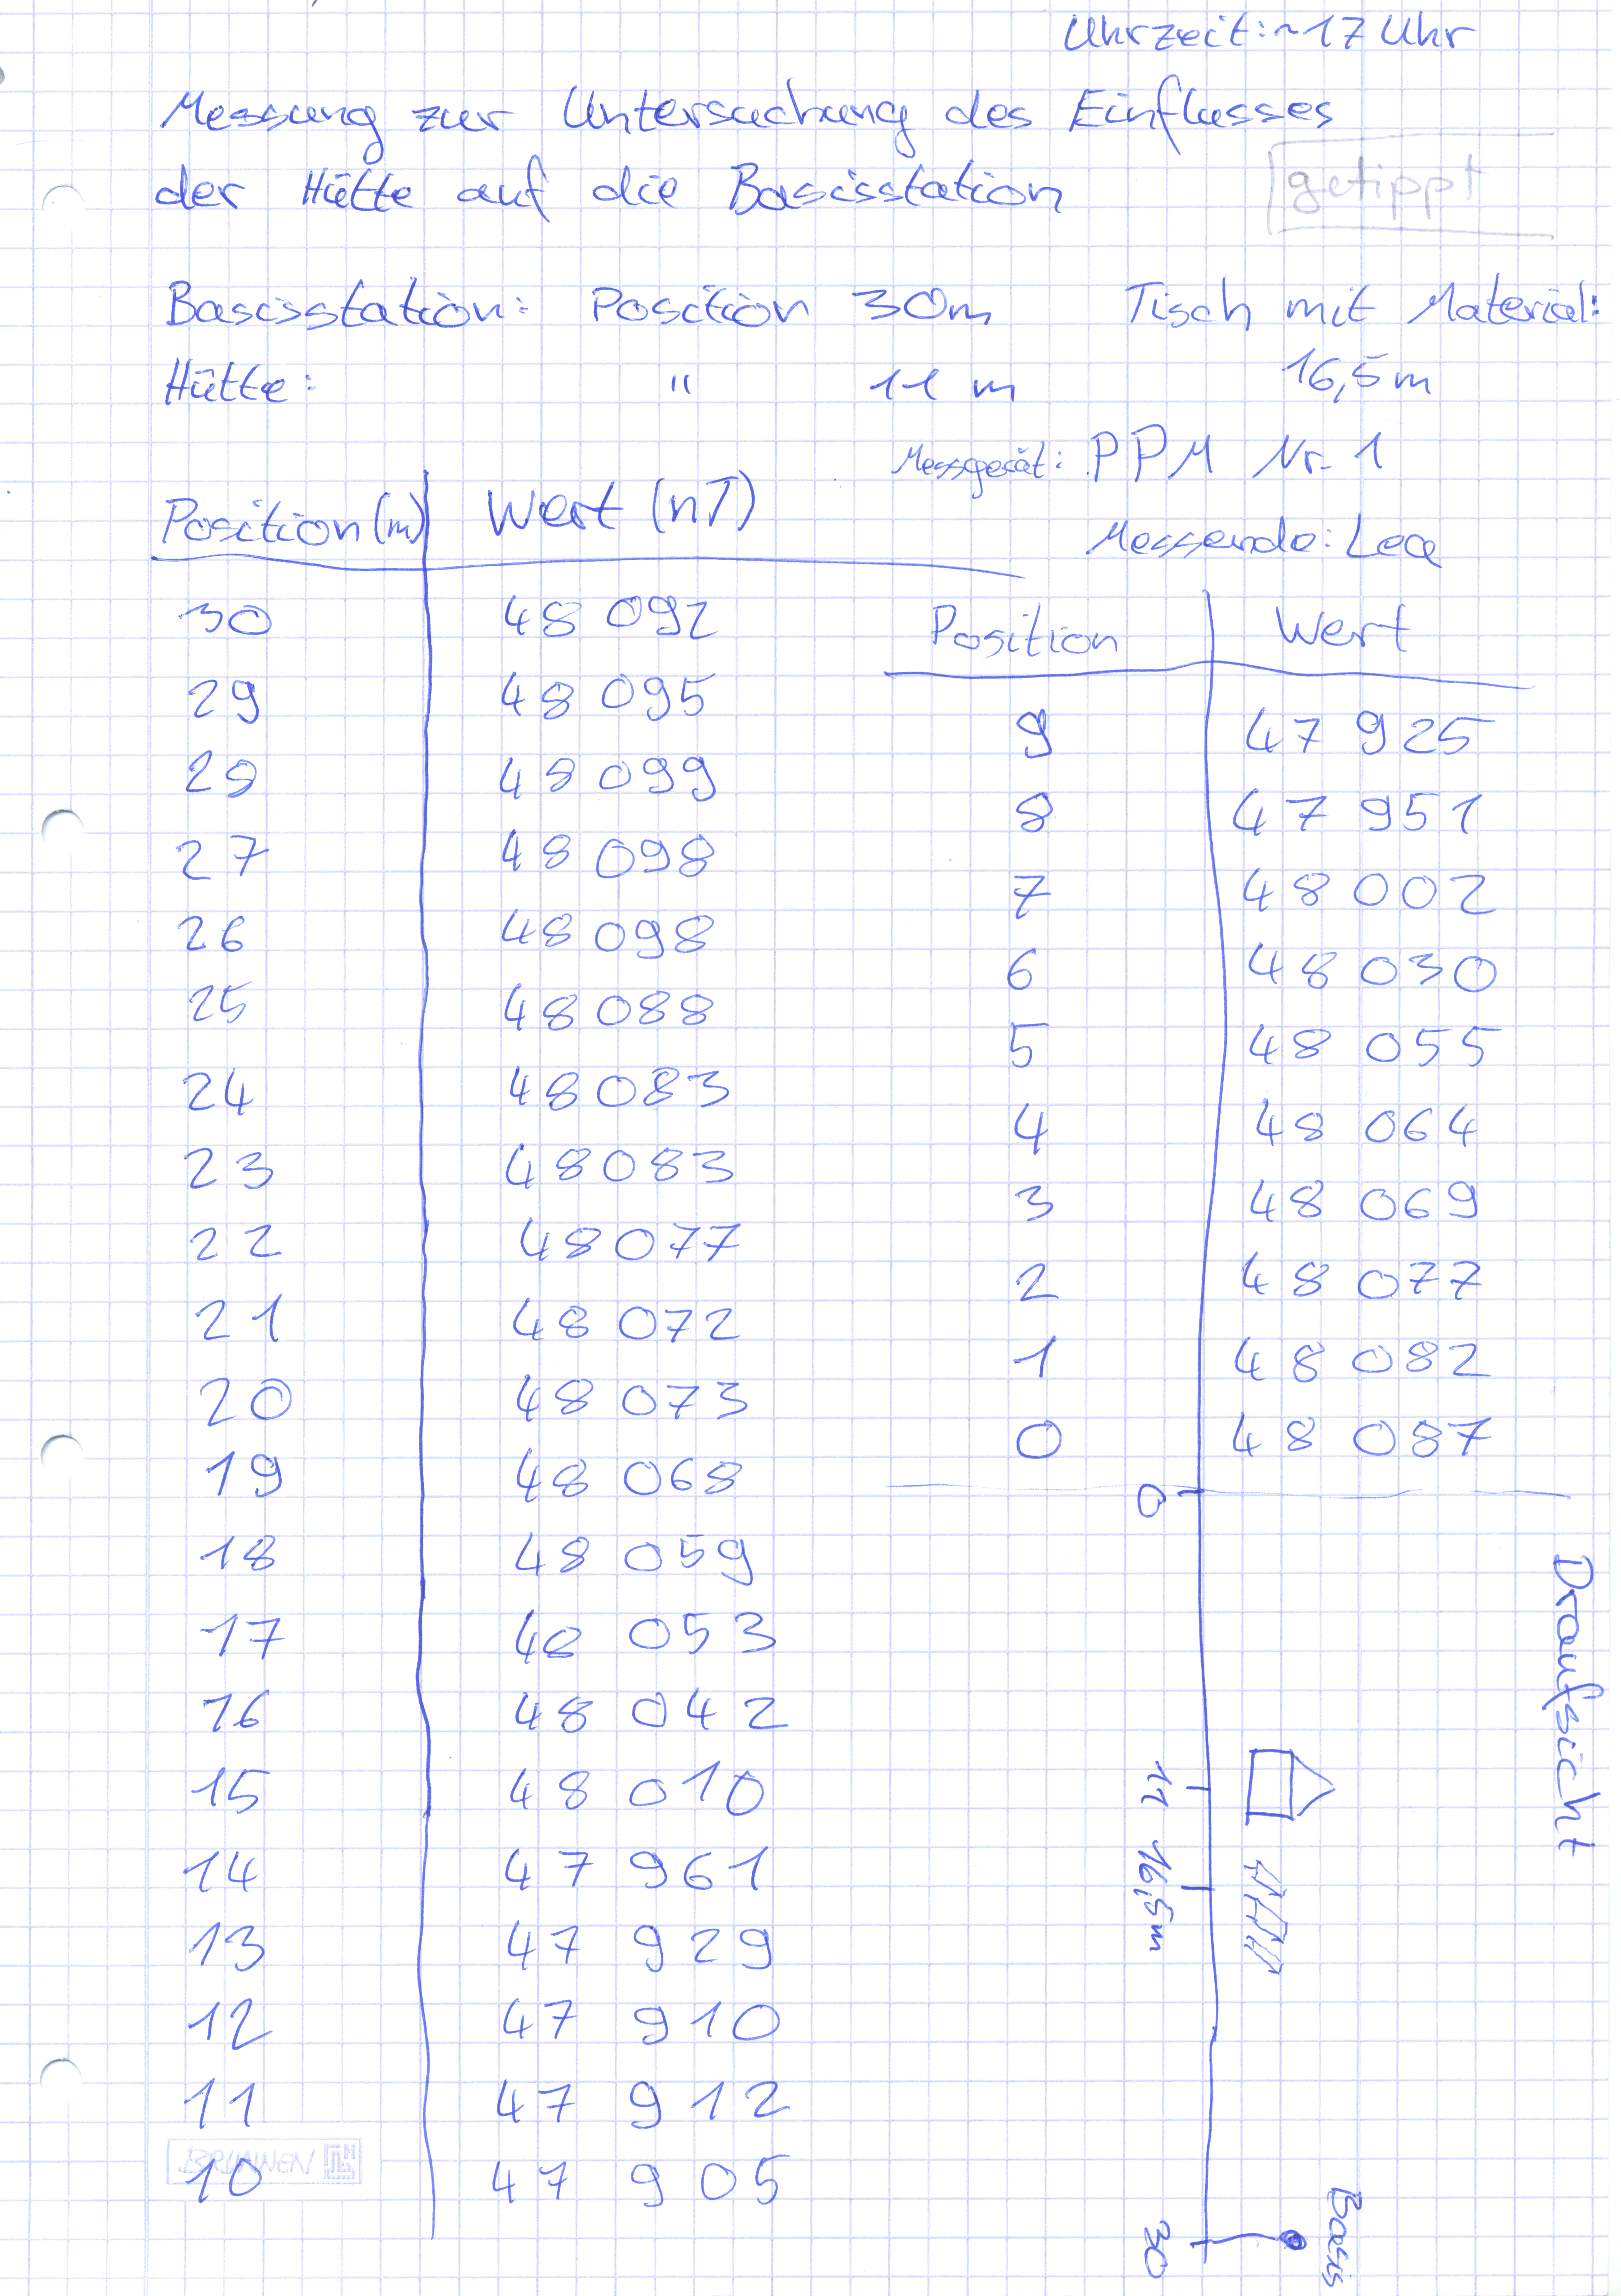
\includegraphics[width=\textwidth]{fig/Messprotokolle/EinflussHuette.png}
 \caption{Messprotokoll zum Profil zur Untersuchung der Einflüsse äußerer Störfaktoren auf die Basismessung}
 \label{fig:MPHuette}
\end{figure}

% \begin{figure}[h!]
%  \centering
%  \includegraphics[width=\textwidth]{fig/Messprotokolle/}
%  \caption{}
%  \label{fig:}
% \end{figure}